\maketitle


\section{The Design Of FactExplorer} 
%在本章节中,我们讨论FactExplorer的设计目标以及System Pipeline,关于系统实现的详细内容将在下一章节阐述。
In this section, we discuss the design goals and system pipeline of FactExplorer. The details of the system implementation will be described in the next section.
\subsection{Design Goals} 
%FactExplorer的主要设计目标是最小化用户的努力去探索并且发现事件空间的有趣模式。更具体地,我们归纳出如下4个目标:
The main design goal of FactExplorer is to minimize users' efforts to explore and discover interesting patterns in the fact space. More specifically, we summarize the following four goals:

%1、确保提取数据事件的质量。系统应该确保提取的事件能覆盖大部分的原始数据空间、确保每个事件包括丰富的数据量、确保事件的可视化样式的多元性
\textbf{G1 Ensure the high quality of data facts.} The system should ensure that the extracted facts can cover most of the original data space, ensure that each fact includes a rich amount of data, and ensure that the visual styles of the facts are diverse.

%2、支持事件空间的语义概述。系统应该建模事件之间的相关性,并提供整个事件空间的概览。以促进用户对一个整体的理解。
\textbf{G2 Support a semantic overview of fact space.} The system should model relationships between facts and provide an overview of the entire fact space to facilitate users to develop a holistic understanding.

%3、将数据事件组织成故事线。系统应该将零散的事件组织成具有一定信息跨度、可视编码相关、逻辑相关的故事线。此外,系统还应该提供指定事件之间的过渡路径来进一步增强探索的灵活性
\textbf{G3 Organize data facts into storylines.} The system should organize fragmented facts into informative, encoding related, and logically related storylines. In addition, system should also provide a transition path between specified facts to incorporate real-time insights from users.

%4、支持便捷的用户交互。系统应该提供灵活的交互,以支持查询、筛选、查看特定的事件集合,并支持对生成数据事实和故事线进行全面编辑,以便用户从自己的视角去探索。
\textbf{G4 Support convenient user interactions.} The system should provide certain flexible interactive components to support querying, filtering, and viewing specific facts, and to enable comprehensive editing of generated facts and storylines for users.
\subsection{System Pipeline} 
%为了达到这些设计目标,我们采用面-线-点的层次结构来呈现数据事件。我们首先从表格数据中提取出事件(点)。然后将这些事件嵌入进事件空间,以使事件集的全局特征被揭露(面)。最后组装相关的事件成有意义的故事线(线)。图1显示了FactExplorer系统的pipline,它由三个核心模块组成
To achieve these design goals, we utilize a \textbf{plane-line-point} hierarchy to present data facts[cite]. We first extract the facts (\textbf{point}) from the tabular data. These facts are then embedded into the fact space to revealed the global features of fact collection (\textbf{plane}). Finally, related facts are assembled into meaningful storylines (\textbf{line}). Figure 1 shows the pipline of the FactExplorer system, which consists of three core modules

%事件提取。常用事件提取方法被采用来从表格数据中提取事件,处理过程包括:子空间切片、事件枚举、事件筛选、事件打分,这些过程都是系统自动完成的不需要用户干预。经过这个模块,底层的原始数据被转换成事件集合。
\textbf{Fact extraction.} Common fact extraction methods are utilized to extract facts from tabular data[cite]. The procedures executed include: subspace slicing, fact enumeration, fact screening, and fact scoring[\textbf{G1}]. These processes are automatically completed by the system , user only need to select the data attributes and fact types that participate in the fact extraction[\textbf{G4}]. After this module, the underlying raw data is converted into an fact collection.

%事件嵌入。在这个模块中,事件被嵌入到事件空间中,以提供一个事件集概览给用户。我们采用多通道嵌入的方法,和事件密切相关的属性(可视编码、逻辑性、偏差)都将被各自嵌入,最后这个单属性通道的嵌入通过不同权重聚合成最终的嵌入表达。
\textbf{Fact embedding.} In this module, facts are embedded into fact space to provide an overview of the fact collection. We adopt the method of multi-channel embedding, and factors closely related to the fact (visual encoding, logical, and deviation) will be embedded separately. Finally, these one-factor embeddings are aggregated into the final embedding by assigning different weights[\textbf{G2, G4}].

%故事线生成。在本模块,我们通过提取故事线来搭起事件间和事件簇间联系的桥梁,从而勾勒出事件空间中的结构。用户可以顺着故事线浏览事件空间中的干线,能够有效促进用户对事件空间的认知,加速探索进程。故事线提取的详细将在下个章节讨论。
\textbf{Storyline generation. }In this module, we delineate the structure in the fact space by extracting storylines to bridge the connections among facts and fact clusters[\textbf{G3}]. Users can browse the trunks along the storyline, it can effectively promote users' cognition of the fact space and accelerate the exploration process. The details of storyline extraction will be discussed in the next section.
\begin{figure}[h]
	\centering
	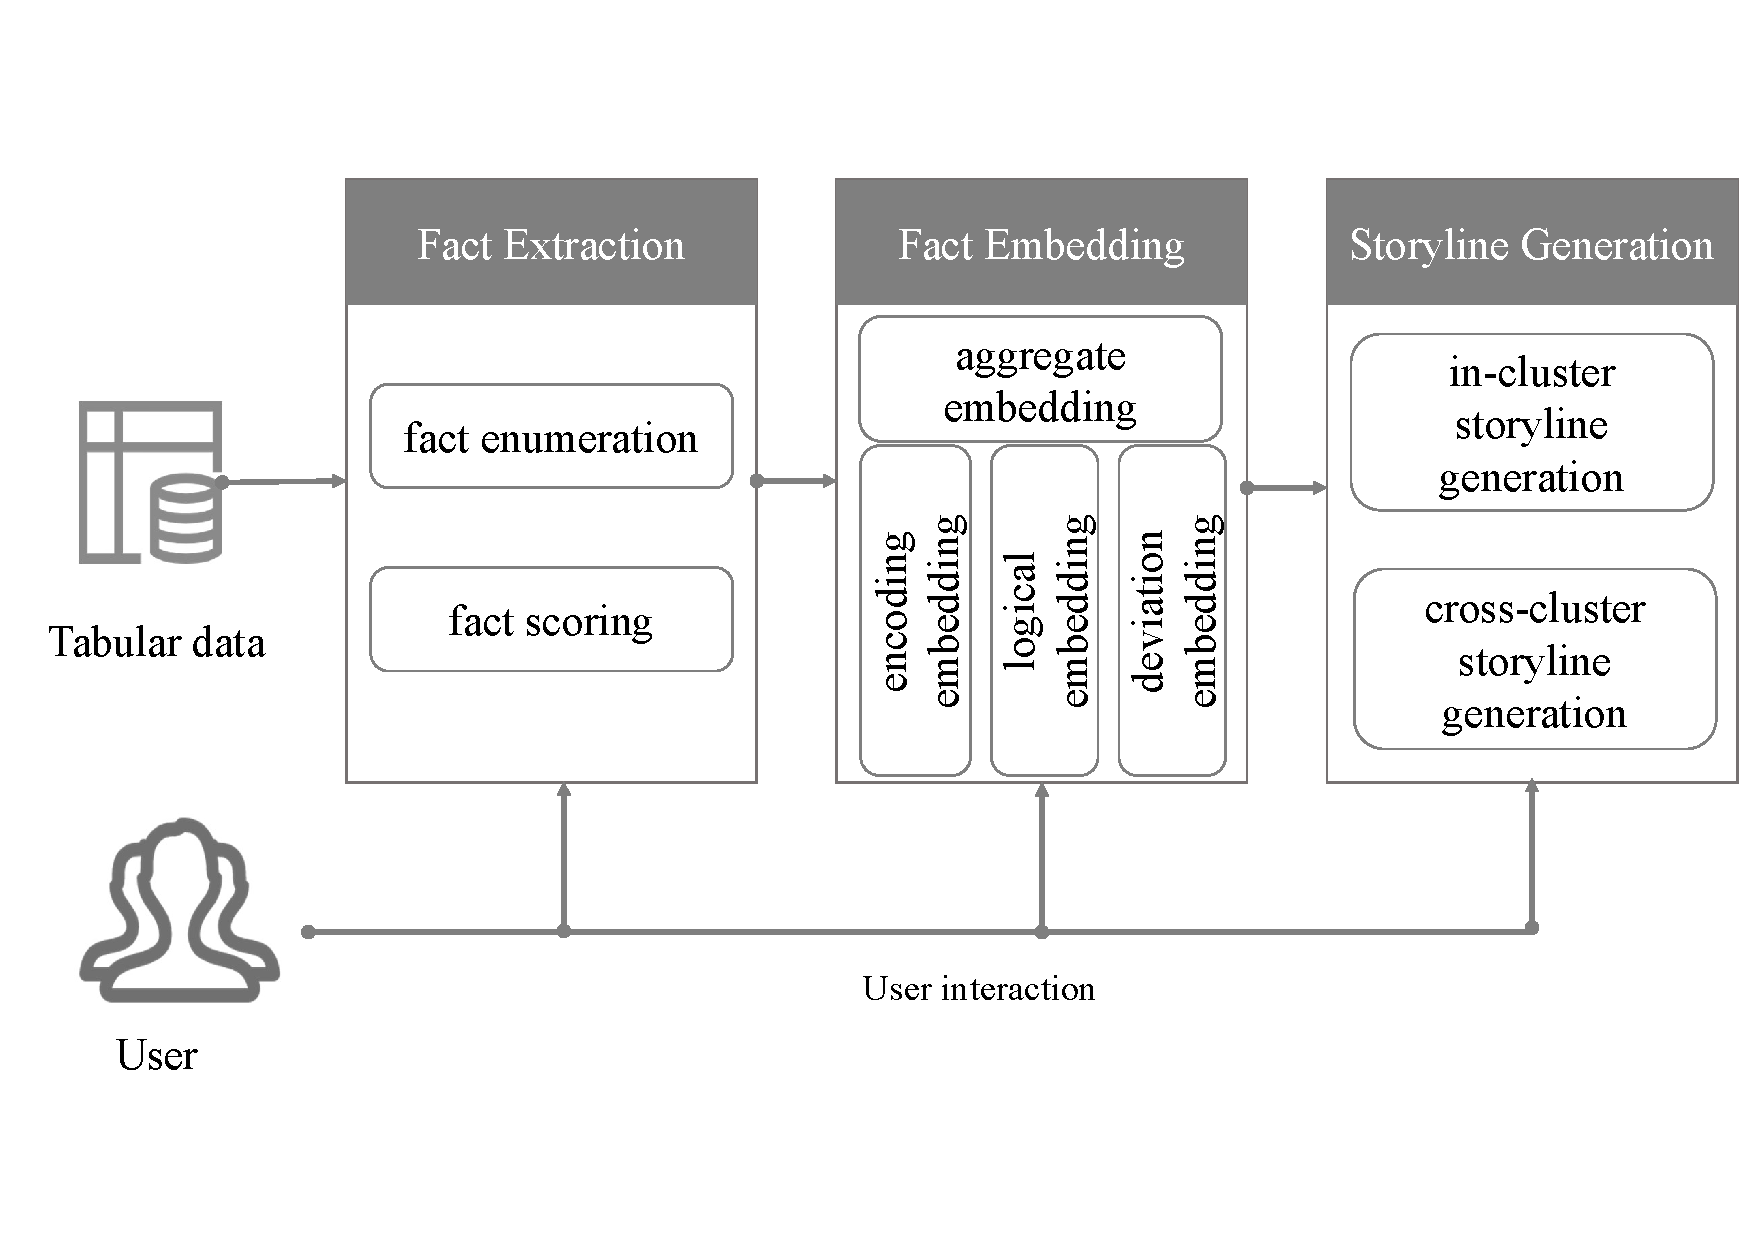
\includegraphics[width=0.5\textwidth]{figures/pipline.pdf}
	\caption{The processing pipeline of FactExplorer. First, FactExplorer automatically extracts facts from the tabular data and scores these facts. Next, these facts will be embedded into fact space from three perspectives: visual encoding, logical, and deviation. Finally, storylines will be extracted after clustering the facts.}
	\label{pipline}
\end{figure}